%% fig1_studyflow.tex — Two-Column Portrait Layout (Journal-Width)
%% Fits standard manuscript text width (~19-20cm) without downscaling.
%% Best practice APA 7: Helvetica / Arial sans-serif typography, clean lines without arrows.
%% Compile with: xelatex fig1_studyflow.tex (or pdflatex fig1_studyflow.tex)

\documentclass[10pt]{article}
\usepackage[paperwidth=21.2cm, paperheight=16.1cm, margin=0.5cm]{geometry}
\usepackage{tikz}
\usepackage{xcolor}
\usepackage{iftex}
\ifxetex
  \usepackage{fontspec}
  \setmainfont{Helvetica}
\else
  \usepackage[utf8]{inputenc}
  \usepackage{amsmath}
  \usepackage{lmodern}
  \renewcommand{\familydefault}{\sfdefault}
\fi
\usepackage{amsmath}
\usepackage{microtype}
\pagestyle{empty}

\usetikzlibrary{arrows.meta, positioning, fit, calc, backgrounds}

%% Palette (Academic publication styling)
\definecolor{Cnavy}{HTML}{1C3A5E}
\definecolor{Cgold}{HTML}{B07D1A}
\definecolor{Cmuted}{HTML}{64748B}
\definecolor{Cspine}{HTML}{94A3B8}
\definecolor{Cblocktxt}{HTML}{1E293B}
\definecolor{Cbg}{HTML}{F8FAFC}
\definecolor{Cborder}{HTML}{CBD5E1}
\definecolor{Cctrl}{HTML}{78909C}
\definecolor{Cadv}{HTML}{A0431E}
\definecolor{Cval}{HTML}{2D7A57}
\definecolor{Cinfo}{HTML}{1E56A0}
\definecolor{Cuserbg}{HTML}{EDF2F7}
\definecolor{Cgptbg}{HTML}{E2EEF9}
\definecolor{Cmetricz}{HTML}{EFF6FF}

\tikzset{
  phasecirc/.style={
    circle, fill=Cgold, text=white,
    minimum size=0.62cm,
    font=\small\bfseries,
    draw=none, inner sep=0pt
  },
  cblock/.style={
    rectangle, rounded corners=3pt,
    fill=white, draw=Cborder, line width=0.5pt,
    align=left, inner sep=5.5pt,
    font=\footnotesize\color{Cblocktxt}
  },
  sbox/.style={
    rectangle, rounded corners=3pt,
    fill=Cbg, draw=Cborder, line width=0.45pt,
    align=left, font=\scriptsize\color{Cblocktxt},
    inner sep=5pt
  },
  condcard/.style={
    rectangle, rounded corners=4pt,
    text=white,
    minimum width=2.02cm, minimum height=1.95cm,
    align=center, font=\scriptsize\bfseries,
    inner sep=2.5pt, draw=none
  },
  sarrow/.style={
    line width=0.8pt, color=Cspine
  },
  fanarrow/.style={
    line width=0.6pt, color=Cspine
  },
  roundbadge/.style={
    anchor=west,
    font=\tiny\bfseries,
    text=Cnavy,
    fill=Cbg,
    draw=Cborder,
    rounded corners=2pt,
    inner sep=2.5pt,
    line width=0.4pt
  },
  chatlabel/.style={
    font=\tiny\bfseries,
    text=Cmuted
  },
  chatbubble/.style={
    rectangle, rounded corners=4pt,
    line width=0.4pt,
    inner sep=5pt,
    align=left,
    font=\scriptsize\color{Cblocktxt}
  }
}

\begin{document}
\noindent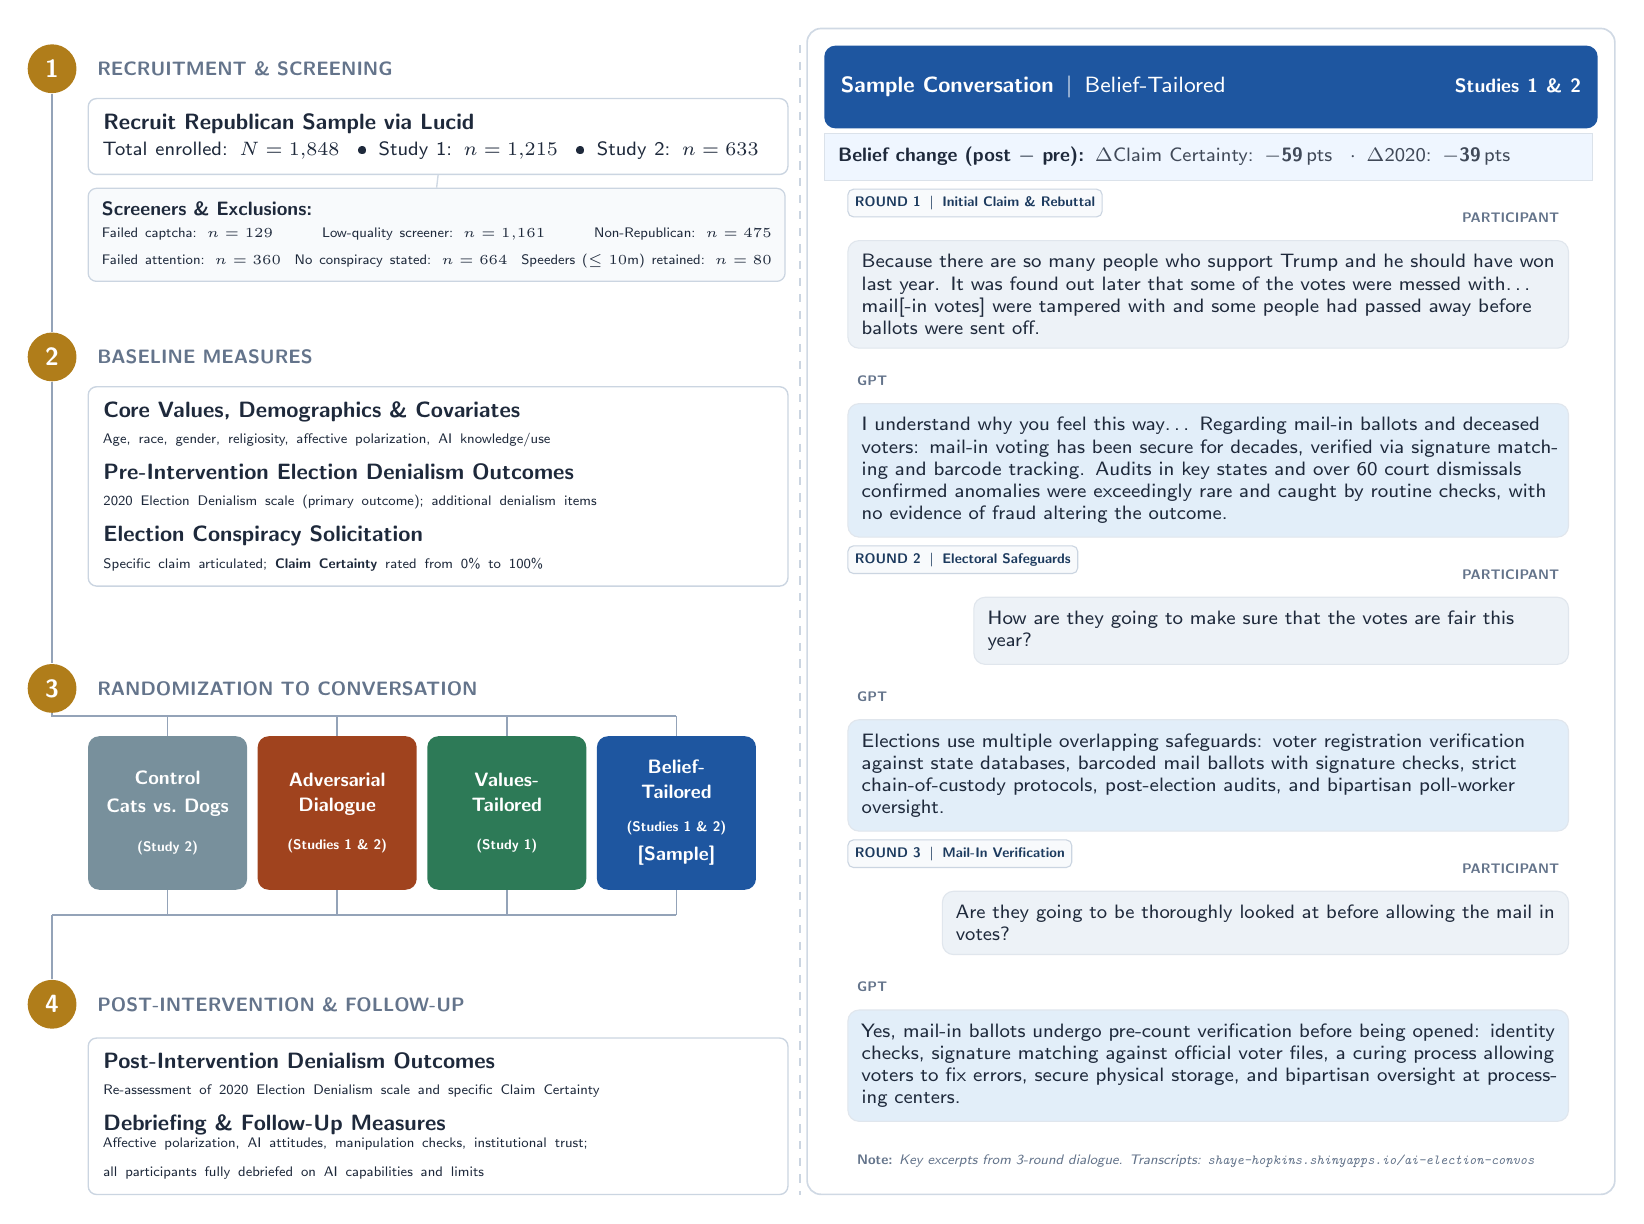
\begin{tikzpicture}

%%════════════════════════════════════════════════════════════
%%  RIGHT COLUMN — SAMPLE DIALOGUE (~9.6cm wide)
%%════════════════════════════════════════════════════════════

%% Header bar
\node[rectangle, rounded corners=4pt,
      fill=Cinfo, text=white,
      text width=9.4cm, minimum height=1.05cm,
      align=left, inner sep=6pt,
      font=\footnotesize\bfseries,
      anchor=north west]
  (cheader) at (10.15, 0.35)
  {Sample Conversation\enspace\textbar\enspace
   \textit{\normalfont\footnotesize Belief-Tailored}%
   \hfill{\scriptsize\normalfont\bfseries Studies 1 \& 2}};

%% Belief-change metric strip
\node[rectangle,
      fill=Cmetricz, draw=Cborder!70, line width=0.4pt,
      text width=9.4cm,
      anchor=north west, inner sep=5pt,
      font=\scriptsize\bfseries\color{Cblocktxt}]
  (cmetric) at ($(cheader.south west)+(0,-0.05cm)$)
  {Belief change (post $-$ pre):\enspace
   \mdseries\color{Cblocktxt!85}%
   $\Delta$Claim Certainty: \textbf{$-$59}\,pts
   \enspace$\cdot$\enspace
   $\Delta$2020: \textbf{$-$39}\,pts};

%% ── ROUND 1 ──
\node[roundbadge] (r1badge) at ($(cmetric.south west)+(0.3cm,-0.28cm)$)
  {ROUND 1\enspace\textbar\enspace Initial Claim \& Rebuttal};

\node[chatlabel, anchor=north east] (u1label) at ($(cmetric.south east)+(-0.3cm,-0.28cm)$)
  {PARTICIPANT};

\node[chatbubble, fill=Cuserbg, draw=Cborder!60, text width=8.8cm, anchor=north east]
  (u1bubble) at ($(u1label.south east)+(0,-0.1cm)$)
  {Because there are so many people who support Trump and he should have won last year. It was found out later that some of the votes were messed with\dots\ mail[-in votes] were tampered with and some people had passed away before ballots were sent off.};

\node[chatlabel, anchor=north west] (g1label) at ($(cmetric.south west |- u1bubble.south)+(0.3cm,-0.22cm)$)
  {GPT};

\node[chatbubble, fill=Cgptbg, draw=Cborder!60, text width=8.8cm, anchor=north west]
  (g1bubble) at ($(g1label.south west)+(0,-0.1cm)$)
  {I understand why you feel this way\dots\ Regarding mail-in ballots and deceased voters: mail-in voting has been secure for decades, verified via signature matching and barcode tracking. Audits in key states and over 60 court dismissals confirmed anomalies were exceedingly rare and caught by routine checks, with no evidence of fraud altering the outcome.};

%% ── ROUND 2 ──
\node[roundbadge] (r2badge) at ($(cmetric.south west |- g1bubble.south)+(0.3cm,-0.28cm)$)
  {ROUND 2\enspace\textbar\enspace Electoral Safeguards};

\node[chatlabel, anchor=north east] (u2label) at ($(cmetric.south east |- g1bubble.south)+(-0.3cm,-0.28cm)$)
  {PARTICIPANT};

\node[chatbubble, fill=Cuserbg, draw=Cborder!60, text width=7.2cm, anchor=north east]
  (u2bubble) at ($(u2label.south east)+(0,-0.1cm)$)
  {How are they going to make sure that the votes are fair this year?};

\node[chatlabel, anchor=north west] (g2label) at ($(cmetric.south west |- u2bubble.south)+(0.3cm,-0.22cm)$)
  {GPT};

\node[chatbubble, fill=Cgptbg, draw=Cborder!60, text width=8.8cm, anchor=north west]
  (g2bubble) at ($(g2label.south west)+(0,-0.1cm)$)
  {Elections use multiple overlapping safeguards: voter registration verification against state databases, barcoded mail ballots with signature checks, strict chain-of-custody protocols, post-election audits, and bipartisan poll-worker oversight.};

%% ── ROUND 3 ──
\node[roundbadge] (r3badge) at ($(cmetric.south west |- g2bubble.south)+(0.3cm,-0.28cm)$)
  {ROUND 3\enspace\textbar\enspace Mail-In Verification};

\node[chatlabel, anchor=north east] (u3label) at ($(cmetric.south east |- g2bubble.south)+(-0.3cm,-0.28cm)$)
  {PARTICIPANT};

\node[chatbubble, fill=Cuserbg, draw=Cborder!60, text width=7.6cm, anchor=north east]
  (u3bubble) at ($(u3label.south east)+(0,-0.1cm)$)
  {Are they going to be thoroughly looked at before allowing the mail in votes?};

\node[chatlabel, anchor=north west] (g3label) at ($(cmetric.south west |- u3bubble.south)+(0.3cm,-0.22cm)$)
  {GPT};

\node[chatbubble, fill=Cgptbg, draw=Cborder!60, text width=8.8cm, anchor=north west]
  (g3bubble) at ($(g3label.south west)+(0,-0.1cm)$)
  {Yes, mail-in ballots undergo pre-count verification before being opened: identity checks, signature matching against official voter files, a curing process allowing voters to fix errors, secure physical storage, and bipartisan oversight at processing centers.};

%% ── Footer note ──
\node[anchor=north west, font=\tiny\itshape, text=Cmuted]
  (rnote) at ($(cmetric.south west |- g3bubble.south)+(0.3cm,-0.30cm)$)
  {\textbf{Note:} Key excerpts from 3-round dialogue. Transcripts: \texttt{shaye-hopkins.shinyapps.io/ai-election-convos}};

%% Outer card border
\begin{pgfonlayer}{background}
  \node[rectangle, rounded corners=5pt,
        fill=white, draw=Cborder!90, line width=0.6pt,
        fit=(cheader)(cmetric)(r1badge)(u1bubble)(g1bubble)(r2badge)(u2bubble)(g2bubble)(r3badge)(u3bubble)(g3bubble)(rnote),
        inner sep=6pt] (cpanel) {};
\end{pgfonlayer}

%% Vertical column divider matching exact panel height
\draw[line width=0.5pt, color=Cborder, dashed]
  let \p1 = (cpanel.south) in (9.85, 0.35) -- (9.85, \y1);


%%════════════════════════════════════════════════════════════
%%  LEFT COLUMN — STUDY DESIGN & PROCEDURE (~9.6cm wide)
%%════════════════════════════════════════════════════════════

%%-- PHASE 1 --%%
\node[phasecirc] (ph1) at (0.35, 0.05) {1};
\node[anchor=west, font=\scriptsize\bfseries, text=Cmuted]
  at (0.8, 0.05) {RECRUITMENT \& SCREENING};

\node[cblock, text width=8.5cm, anchor=north west] (rec) at (0.8, -0.32)
  {\textbf{Recruit Republican Sample via Lucid}\\
   {\scriptsize Total enrolled: $N = 1{,}848$ \enspace\textbullet\enspace Study 1: $n = 1{,}215$ \enspace\textbullet\enspace Study 2: $n = 633$}};

\node[sbox, text width=8.5cm, anchor=north west] (sbox) at ($(rec.south west)+(0,-0.16cm)$)
  {\textbf{Screeners \& Exclusions:}\\[2pt]
   {\tiny
   Failed captcha: $n=129$ \hfill Low-quality screener: $n=1{,}161$ \hfill Non-Republican: $n=475$\\[1.5pt]
   Failed attention: $n=360$ \hfill No conspiracy stated: $n=664$ \hfill Speeders ($\le 10$m) retained: $n=80$}};

\draw[line width=0.5pt, color=Cborder!90] (rec.south) -- (sbox.north);

%%-- PHASE 2 --%%
\node[phasecirc] (ph2) at (0.35, -3.61) {2};
\draw[sarrow] (ph1.south) -- (ph2.north);
\node[anchor=west, font=\scriptsize\bfseries, text=Cmuted]
  at (0.8, -3.61) {BASELINE MEASURES};

\node[cblock, text width=8.5cm, anchor=north west] (base) at (0.8, -3.98)
  {\textbf{Core Values, Demographics \& Covariates}\\
   {\tiny Age, race, gender, religiosity, affective polarization, AI knowledge/use}\\[3.5pt]
   \textbf{Pre-Intervention Election Denialism Outcomes}\\
   {\tiny 2020 Election Denialism scale (primary outcome); additional denialism items}\\[3.5pt]
   \textbf{Election Conspiracy Solicitation}\\
   {\tiny Specific claim articulated; \textbf{Claim Certainty} rated from 0\% to 100\%}};

%%-- PHASE 3 --%%
\node[phasecirc] (ph3) at (0.35, -7.82) {3};
\draw[sarrow] (ph2.south) -- (ph3.north);
\node[anchor=west, font=\scriptsize\bfseries, text=Cmuted]
  at (0.8, -7.82) {RANDOMIZATION TO CONVERSATION};

\node[condcard, fill=Cctrl, anchor=north west] (c1) at (0.8, -8.42)
  {\textbf{Control}\\[2pt]{\scriptsize\color{white!90}Cats vs.~Dogs}\\[6pt]{\tiny\color{white!75}(Study 2)}};

\node[condcard, fill=Cadv, right=0.12cm of c1] (c2)
  {\textbf{Adversarial}\\[1pt]\textbf{Dialogue}\\[6pt]{\tiny\color{white!75}(Studies 1 \& 2)}};

\node[condcard, fill=Cval, right=0.12cm of c2] (c3)
  {\textbf{Values-}\\[1pt]\textbf{Tailored}\\[6pt]{\tiny\color{white!75}(Study 1)}};

\node[condcard, fill=Cinfo, right=0.12cm of c3] (c4)
  {\textbf{Belief-}\\[1pt]\textbf{Tailored}\\[4pt]{\tiny\color{white!75}(Studies 1 \& 2)}\\[2.5pt]{\scriptsize\bfseries\color{white}[Sample]}};

%% Fan-out: spine -> horizontal bar -> card tops (clean lines, no arrows)
\draw[line width=0.8pt, color=Cspine]
  (ph3.south) -- (0.35, -8.17) -- (c4.north |- 0.35, -8.17);
\foreach \cnode in {c1, c2, c3, c4}{
  \draw[fanarrow] (\cnode.north |- 0.35, -8.17) -- (\cnode.north);
}

%% Fan-in: card bottoms -> collector bar -> spine (clean lines, no arrows)
\draw[line width=0.8pt, color=Cspine]
  (c4.south |- 0.35, -10.70) -- (0.35, -10.70);
\foreach \cnode in {c1, c2, c3, c4}{
  \draw[fanarrow] (\cnode.south) -- (\cnode.south |- 0.35, -10.70);
}

%%-- PHASE 4 --%%
%% Anchor post.south directly to cpanel.south for exact pixel-aligned bottom!
\node[cblock, text width=8.5cm, anchor=south west] (post) at (0.8, 0 |- cpanel.south)
  {\textbf{Post-Intervention Denialism Outcomes}\\
   {\tiny Re-assessment of 2020 Election Denialism scale and specific Claim Certainty}\\[3.5pt]
   \textbf{Debriefing \& Follow-Up Measures}\\
   {\tiny Affective polarization, AI attitudes, manipulation checks, institutional trust;\\[1pt]
    all participants fully debriefed on AI capabilities and limits}};

\node[phasecirc] (ph4) at ($(post.north -| 0.35, 0)+(0, 0.42cm)$) {4};
\draw[sarrow] (0.35, -10.70) -- (ph4.north);
\node[anchor=west, font=\scriptsize\bfseries, text=Cmuted]
  at (0.8, 0 |- ph4) {POST-INTERVENTION \& FOLLOW-UP};

\end{tikzpicture}
\end{document}
